\documentclass[compress]{beamer}

%Importando alguns pacotes
\usepackage{lipsum}
\usepackage{fancyvrb}
\usepackage{ragged2e}
\usepackage{xcolor}
%\usepackage{default}
\usepackage{graphicx}
\usepackage{tikz}
\usepackage[alf]{abntex2cite}

%Importando alguns pacotes
\usepackage{appendixnumberbeamer}
\usepackage{booktabs}
\usepackage[scale=2]{ccicons}

%Importando alguns pacotes
\usepackage{pgfplots}
\usepgfplotslibrary{dateplot}

%Importando alguns pacotes e criando um novo comando
\usepackage{xspace}
\newcommand{\themename}{\textbf{\textsc{metropolis}}\xspace}


%Usando tikz
\usetikzlibrary{positioning}
%\usepgflibrary{decorations.pathreplacing}
\usetikzlibrary{decorations.pathreplacing}
\usetikzlibrary{decorations.pathmorphing}
\usetikzlibrary[patterns]
%\tikzstyle{every text node part}
%\usetikzlibrary{arrows,backgrounds,positioning,fit} 
\usetikzlibrary{calc}

% para gerar graficos no latex
\usepackage{pgfplots}
\pgfplotsset{compat=newest}

%Importando alguns pacotes
\usepackage[newfloat]{minted}
\usepackage{caption}
\usemintedstyle{borland}
\usepackage{amsfonts}
\usepackage{amssymb}
\usepackage{amsmath}
\usepackage{MnSymbol}
\usepackage[brazilian]{babel}
\usepackage[utf8]{inputenc}
\usepackage[Algoritmo]{algorithm}
\usepackage[noend]{algorithmic}

\usepackage[brazilian,hyperpageref]{backref}	 % Paginas com as citações na bibl
\usepackage[alf]{abntex2cite}	% Citações padrão ABNT

%Setando bibliografia beamer
% \setbeamertemplate{bibliography entry title}{}
% \setbeamertemplate{bibliography entry location}{}
% \setbeamertemplate{bibliography entry note}{}

\newcounter{saveenumi}
\newcommand{\seti}{\setcounter{saveenumi}{\value{enumi}}}
\newcommand{\conti}{\setcounter{enumi}{\value{saveenumi}}}

%\usepackage{shadethm}

%\definecolor{shadethmcolor}{rgb}{.75,.75,.75}

%Definindo novas cores
\definecolor{LightGray}{gray}{0.95}
\definecolor{shadecolor}{rgb}{.9, .9, .9}

%\newshadetheorem{theorem}{\scshape Teorema}[chapter]
\newtheorem{teorema}[theorem]{\scshape Teorema}
\newtheorem{proposicao}[theorem]{\scshape Proposição}
\newtheorem{corolario}[theorem]{\scshape Corolário}
\newtheorem{lema}[theorem]{\scshape Lema}
\newtheorem{definicao}[theorem]{\scshape Definição}
\newtheorem{conjectura}[theorem]{\scshape Conjectura}
\newtheorem{escolio}[theorem]{\scshape Escólio}
\newtheorem{exemplo}[theorem]{\scshape Exemplo}
\newtheorem{exemplos}[theorem]{\scshape Exemplos}
\newtheorem{propriedade}[theorem]{\scshape Propriedade}

\renewcommand{\u}{{\bf u}}
\renewcommand{\v}{{\bf v}}
\renewcommand{\sin}{\operatorname{sen}}
\renewcommand{\tan}{\operatorname{tg}}
\providecommand{\cas}{\operatorname{cas}}
\providecommand{\mdc}{\mathrm{mdc}}
\providecommand{\f}{{\bf f}}

\newcommand{\ie}{\textit{i.e.}}
\newcommand{\eg}{\textit{e.g.}}
%\newcommand{\qed}{\hfill $\square$}

\renewcommand\Re{\operatorname{Re}}
\renewcommand\Im{\operatorname{Im}}

\providecommand{\x}{{\bf x}}
\providecommand{\y}{{\bf y}}
\providecommand{\w}{{\bf w}}
\providecommand{\f}{{\bf f}}
\providecommand{\q}{{\bf q}}
\providecommand{\bfa}{{\bf a}}
\providecommand{\bfb}{{\bf b}}
\providecommand{\bfc}{{\bf c}}
\providecommand{\bfd}{{\bf d}}
\providecommand{\bfe}{{\bf e}}
\providecommand{\bfs}{{\bf s}}
\providecommand{\bfz}{{\bf z}}
\providecommand{\zero}{{\bf 0}}
\providecommand{\spn}{\mathrm{span}}
\providecommand{\posto}{\mathrm{posto}}
\providecommand{\nul}{\mathrm{nul}}
\providecommand{\proj}{\mathrm{proj}}
\providecommand{\tr}{\mathrm{tr}}
\providecommand{\sgn}{\mathrm{sgn}}

\providecommand{\cov}{\mathrm{cov}}

\providecommand{\dilation}{\mathcal{D}}
\providecommand{\erosion}{\mathcal{E}}
\providecommand{\open}{\mathcal{O}}
\providecommand{\close}{\mathcal{C}}

\newcommand*{\Bhat}{\skew{3}{\hat}{B}}

%\usetheme{AnnArbor}
%\usetheme{Antibes}
%\usetheme{Bergen}
%\usetheme{Berkeley}
%\usetheme{Berlin}
%\usetheme{Boadilla}
%\usetheme{boxes}
%\usetheme{CambridgeUS}
%\usetheme{Copenhagen}
%\usetheme{Darmstadt}
%\usetheme{default}
%\usetheme{Frankfurt}
%\usetheme{Goettingen}
%\usetheme{Hannover}
%\usetheme{Ilmenau}
%\usetheme{JuanLesPins}
%\usetheme{Luebeck}
%\usetheme{Madrid}
%\usetheme{Malmoe}
%\usetheme{Marburg}
%\usetheme{Montpellier}
%\usetheme{PaloAlto}
%\usetheme{Pittsburgh}
%\usetheme{Rochester}
%\usetheme{Singapore}
%\usetheme{Szeged}
%\usetheme{Warsaw}
\usetheme{metropolis}

% copiado do site:
% http://latex-beamer-class.10966.n7.nabble.com/Covering-images-transparent-i-e-dimmed-figures-td1504.html
\usepackage{ifthen}

\makeatletter
\newcommand{\includecoveredgraphics}[2][]{
    \ifthenelse{\the\beamer@coveringdepth=1}{
        \tikz
            \node[inner sep=0pt,outer sep=0pt,opacity=0.15]
                {\includegraphics[#1]{#2}};
    }{
        \tikz
            \node[inner sep=0pt,outer sep=0pt]
                {\includegraphics[#1]{#2}};%
    }
} 
\makeatother


% Definindo novas cores para utilizar código
\definecolor{verde}{rgb}{0,0.5,0}
% Configurando layout para mostrar codigos C++
\usepackage{listings}
\lstset{
  language=C++,
  basicstyle=\ttfamily\small,
  keywordstyle=\color{blue},
  stringstyle=\color{verde},
  commentstyle=\color{red},
  extendedchars=true,
  showspaces=false,
  showstringspaces=false,
  numbers=left,
  numberstyle=\tiny,
  breaklines=true,
  backgroundcolor=\color{green!10},
  breakautoindent=true,
  captionpos=b,
  xleftmargin=5pt,
}

\newenvironment{code}{\captionsetup{type=listing}}{}
\SetupFloatingEnvironment{listing}{name=Código Fonte}

%%%%%%%%%%%%%%%%%%%%%%%%%%%%%%%%%%%%%%%%%%%%%%%%%%%%%%%%
%Definindo informações da apresentação                 %
%%%%%%%%%%%%%%%%%%%%%%%%%%%%%%%%%%%%%%%%%%%%%%%%%%%%%%%%

%Definindo Título
\title{Desenvolvimento de um Sistema Web de Apoio à Avaliação Psicopedagógica na Educação Infantil}
%\subtitle{Um modelo de apresentação}
%Definindo Instituição
\institute{Curso de Engenharia da Computação - UEMG - Unidade Divinópolis}
%Definindo autores
\author{Sanielle Gonçalves Azara \and \\
Orientadora: Profa. Ma. Fernanda Rodrigues Macedo}
%Definindo data (pode ser colocada manualmente
\date{25 de novembro de 2026}
%Colocando logo da UEMG
\titlegraphic{\hfill
\includegraphics[height=2cm]{figuras/UEMG_vertical.jpg}}

\begin{document}

% Tempo estimado: ~20 minutos (cerca de 40 a 50 segundos por slide)

\maketitle

\begin{frame}{Sumário}
    \tableofcontents
\end{frame}

%%%%%%%%%%%%%%%%%%%%%%%%%%%%%%%%%%%%%%%%%%%%%%%%%%%%%%%%
\section{Introdução}
%%%%%%%%%%%%%%%%%%%%%%%%%%%%%%%%%%%%%%%%%%%%%%%%%%%%%%%%

\begin{frame}{Contextualização}
\begin{itemize}
    \item A avaliação psicopedagógica busca compreender como fatores cognitivos, emocionais, sociais e contextuais interferem na aprendizagem.
    \item Articula instrumentos, observações e a história do aprendente, e acompanha a criança ao longo do tempo.
    \item Na prática, os registros ainda ficam em papel, planilhas e documentos dispersos.
    \item Consequências: pouca padronização, baixa rastreabilidade e dificuldade de acompanhar a evolução da criança.
    \item Os profissionais adaptam protocolos para cada criança, mas não têm como registrar essas adaptações.
\end{itemize}
\end{frame}

\begin{frame}{Justificativa}
\begin{itemize}
    \item Prontuários eletrônicos do mercado priorizam a gestão do consultório (agenda, financeiro, documentos).
    \item Oferecem, no máximo, instrumentos fixos ou formulários genéricos.
    \item Nenhum informa permitir que o profissional \textbf{cadastre e adapte seus próprios instrumentos} com um \textbf{controle de versões} que preserve a versão usada em cada aplicação.
    \item Conclusões psicopedagógicas são interpretativas: é preciso reunir dados estruturados e espaço para relatórios em texto livre.
\end{itemize}
\end{frame}

\begin{frame}{Objetivo Geral}
Desenvolver um sistema web multiusuário de apoio à avaliação psicopedagógica na Educação Infantil que permita o registro estruturado das informações dos aprendentes, o gerenciamento dos instrumentos avaliativos e o acompanhamento das etapas da avaliação, contribuindo para a padronização, a rastreabilidade e a qualidade das devolutivas.
\end{frame}

\begin{frame}{Objetivos Específicos}
\begin{enumerate}
    \small
    \item Identificar os principais instrumentos e procedimentos da avaliação psicopedagógica infantil.
    \item Projetar a arquitetura do sistema e seus módulos.
    \item Implementar mecanismos de proteção das informações e analisar a adequação à LGPD.
    \item Desenvolver uma interface orientada à usabilidade e à acessibilidade.
    \item Avaliar o sistema com profissionais da psicopedagogia.
    \item Discutir contribuições e limitações em relação aos trabalhos relacionados.
\end{enumerate}
\end{frame}

%%%%%%%%%%%%%%%%%%%%%%%%%%%%%%%%%%%%%%%%%%%%%%%%%%%%%%%%
\section{Estudos Relacionados}
%%%%%%%%%%%%%%%%%%%%%%%%%%%%%%%%%%%%%%%%%%%%%%%%%%%%%%%%

\begin{frame}{Estudos Relacionados}
Buscas na SciELO, PePSIC e BDTD (2013--2025), organizadas em linhas:
\begin{itemize}
    \small
    \item \textbf{Prontuários eletrônicos:} Sistema PSI (Silva et al., 2020) registra sessões, sem estruturar instrumentos; Valgas (2021), o mais próximo, usa DSR na neuropsicologia hospitalar de adultos.
    \item \textbf{Triagem digital do desenvolvimento:} TEDI (Moreira et al., 2022) e ASQ-3 \textit{web} (Schonhaut et al., 2023) digitalizam \textbf{instrumentos fixos}.
    \item \textbf{\textit{Software} na avaliação psicopedagógica:} Pinheiro (2013) usa um instrumento de avaliação e aponta a falta de registro em prontuário.
    \item \textbf{Revisões em saúde mental:} participação dos usuários no projeto (Zurynski et al., 2021) e tensão entre campos estruturados e registro narrativo (Kariotis et al., 2022).
\end{itemize}
\end{frame}

\begin{frame}{Soluções Existentes no Mercado}
\footnotesize
\centering
\begin{tabular}{p{2.1cm}p{3.0cm}p{2.0cm}p{2.0cm}}
\toprule
\textbf{Produto} & \textbf{Instrumentos} & \textbf{Criação própria} & \textbf{Versão na aplicação} \\
\midrule
iPsy Pro & Não & Não informado & Não informado \\
Cerebraris & Conjunto predefinido & Não informado & Não informado \\
PsicoManager & Escalas & Não informado & Não informado \\
Ninsaúde Clinic & Formulários & Sim (modelos) & Não informado \\
\midrule
\textbf{Sistema proposto} & \textbf{Cadastrados pelo profissional} & \textbf{Sim} & \textbf{Sim} \\
\bottomrule
\end{tabular}

\vspace{0.4cm}
\raggedright
\small Fonte: funcionalidades divulgadas nos sítios oficiais (nov. 2026).
\end{frame}

\begin{frame}{Delimitação da Lacuna}
Nenhum estudo ou produto analisado reúne, na avaliação psicopedagógica infantil:
\begin{itemize}
    \item cadastro de instrumentos pelo próprio profissional;
    \item versionamento que preserve a versão usada em cada aplicação;
    \item registro das respostas;
    \item relatórios qualitativos vinculados à aplicação.
\end{itemize}
\vspace{0.3cm}
\textbf{Orientações da literatura:} participação dos profissionais no projeto e equilíbrio entre campos estruturados e registro narrativo.
\end{frame}

%%%%%%%%%%%%%%%%%%%%%%%%%%%%%%%%%%%%%%%%%%%%%%%%%%%%%%%%
\section{Fundamentação Teórica}
%%%%%%%%%%%%%%%%%%%%%%%%%%%%%%%%%%%%%%%%%%%%%%%%%%%%%%%%

\begin{frame}{Fundamentação Teórica}
\begin{columns}[T]
\begin{column}{0.5\textwidth}
\textbf{Psicopedagogia}
\begin{itemize}
    \small
    \item Desenvolvimento infantil de 0 a 6 anos.
    \item Etapas: entrevista, anamnese, observação (EOCA), instrumentos, análise, devolutiva e acompanhamento.
    \item Instrumentos: Portage, IDADI, Denver II, PRELEC.
    \item Adaptações devem ser registradas.
\end{itemize}
\end{column}
\begin{column}{0.5\textwidth}
\textbf{Engenharia de Software}
\begin{itemize}
    \small
    \item Engenharia de requisitos e UML.
    \item Arquitetura em camadas e REST.
    \item Banco relacional e ORM.
    \item JWT e controle de acesso por papéis (RBAC).
    \item Testes de software e WCAG.
\end{itemize}
\end{column}
\end{columns}
\end{frame}

%%%%%%%%%%%%%%%%%%%%%%%%%%%%%%%%%%%%%%%%%%%%%%%%%%%%%%%%
\section{Materiais e Métodos}
%%%%%%%%%%%%%%%%%%%%%%%%%%%%%%%%%%%%%%%%%%%%%%%%%%%%%%%%

\begin{frame}{Classificação da Pesquisa}
Pesquisa aplicada, conduzida segundo a \textit{Design Science Research} (DSR):
\vspace{0.2cm}

\footnotesize
\centering
\begin{tabular}{p{4.0cm}p{6.0cm}}
\toprule
\textbf{Etapa da DSR} & \textbf{Atividade realizada} \\
\midrule
Identificação do problema & Revisão da literatura, mercado e entrevista \\
Projeto do artefato & Requisitos, arquitetura e modelo de dados \\
Desenvolvimento & Implementação incremental e iterativa \\
Avaliação & Testes, acessibilidade e questionário \\
Comunicação & Discussão, limitações e trabalhos futuros \\
\bottomrule
\end{tabular}
\end{frame}

\begin{frame}{Coleta de Dados}
\begin{itemize}
    \item Revisão bibliográfica e análise documental de instrumentos (sem reproduzir seu conteúdo).
    \item Entrevista semiestruturada com uma psicopedagoga (março de 2026), com TCLE:
    \begin{itemize}
        \small
        \item registros em planilhas e documentos sem integração;
        \item dificuldade de manter o histórico longitudinal;
        \item adaptação de protocolos sem registro das versões;
        \item relatórios flexíveis e sigilo restrito ao profissional responsável.
    \end{itemize}
    \item Dados exclusivamente fictícios no ambiente de demonstração.
\end{itemize}
\end{frame}

\begin{frame}{Ferramentas e Tecnologias}
\begin{itemize}
    \item \textbf{\textit{Frontend}:} React, Vite, Material UI, TanStack Query.
    \item \textbf{\textit{Backend}:} Node.js, Express, API REST, JWT, bcrypt.
    \item \textbf{Validação compartilhada:} Zod.
    \item \textbf{Persistência:} MySQL e Prisma.
    \item \textbf{Testes:} Vitest, Supertest, React Testing Library, axe-core e Playwright.
    \item \textbf{Implantação:} Docker e Nginx; Git e GitHub.
\end{itemize}
\end{frame}

%%%%%%%%%%%%%%%%%%%%%%%%%%%%%%%%%%%%%%%%%%%%%%%%%%%%%%%%
\section{Desenvolvimento}
%%%%%%%%%%%%%%%%%%%%%%%%%%%%%%%%%%%%%%%%%%%%%%%%%%%%%%%%

\begin{frame}{Requisitos}
\begin{columns}[T]
\begin{column}{0.5\textwidth}
\textbf{15 requisitos funcionais}
\begin{itemize}
    \small
    \item Cadastro de aprendentes.
    \item Cadastro, versionamento e aplicação de instrumentos.
    \item Histórico e relatórios em PDF.
    \item Visibilidade restrita ao responsável.
\end{itemize}
\end{column}
\begin{column}{0.5\textwidth}
\textbf{11 requisitos não funcionais}
\begin{itemize}
    \small
    \item Autenticação, autorização e auditoria.
    \item Usabilidade: média $\geq$ 4,0.
    \item Cobertura de testes $\geq$ 70\%.
    \item Sem violações WCAG 2.2 (A e AA) detectáveis pelo axe-core.
\end{itemize}
\end{column}
\end{columns}
\end{frame}

\begin{frame}{Arquitetura do Sistema}
\begin{columns}[c]
\begin{column}{0.42\textwidth}
\centering
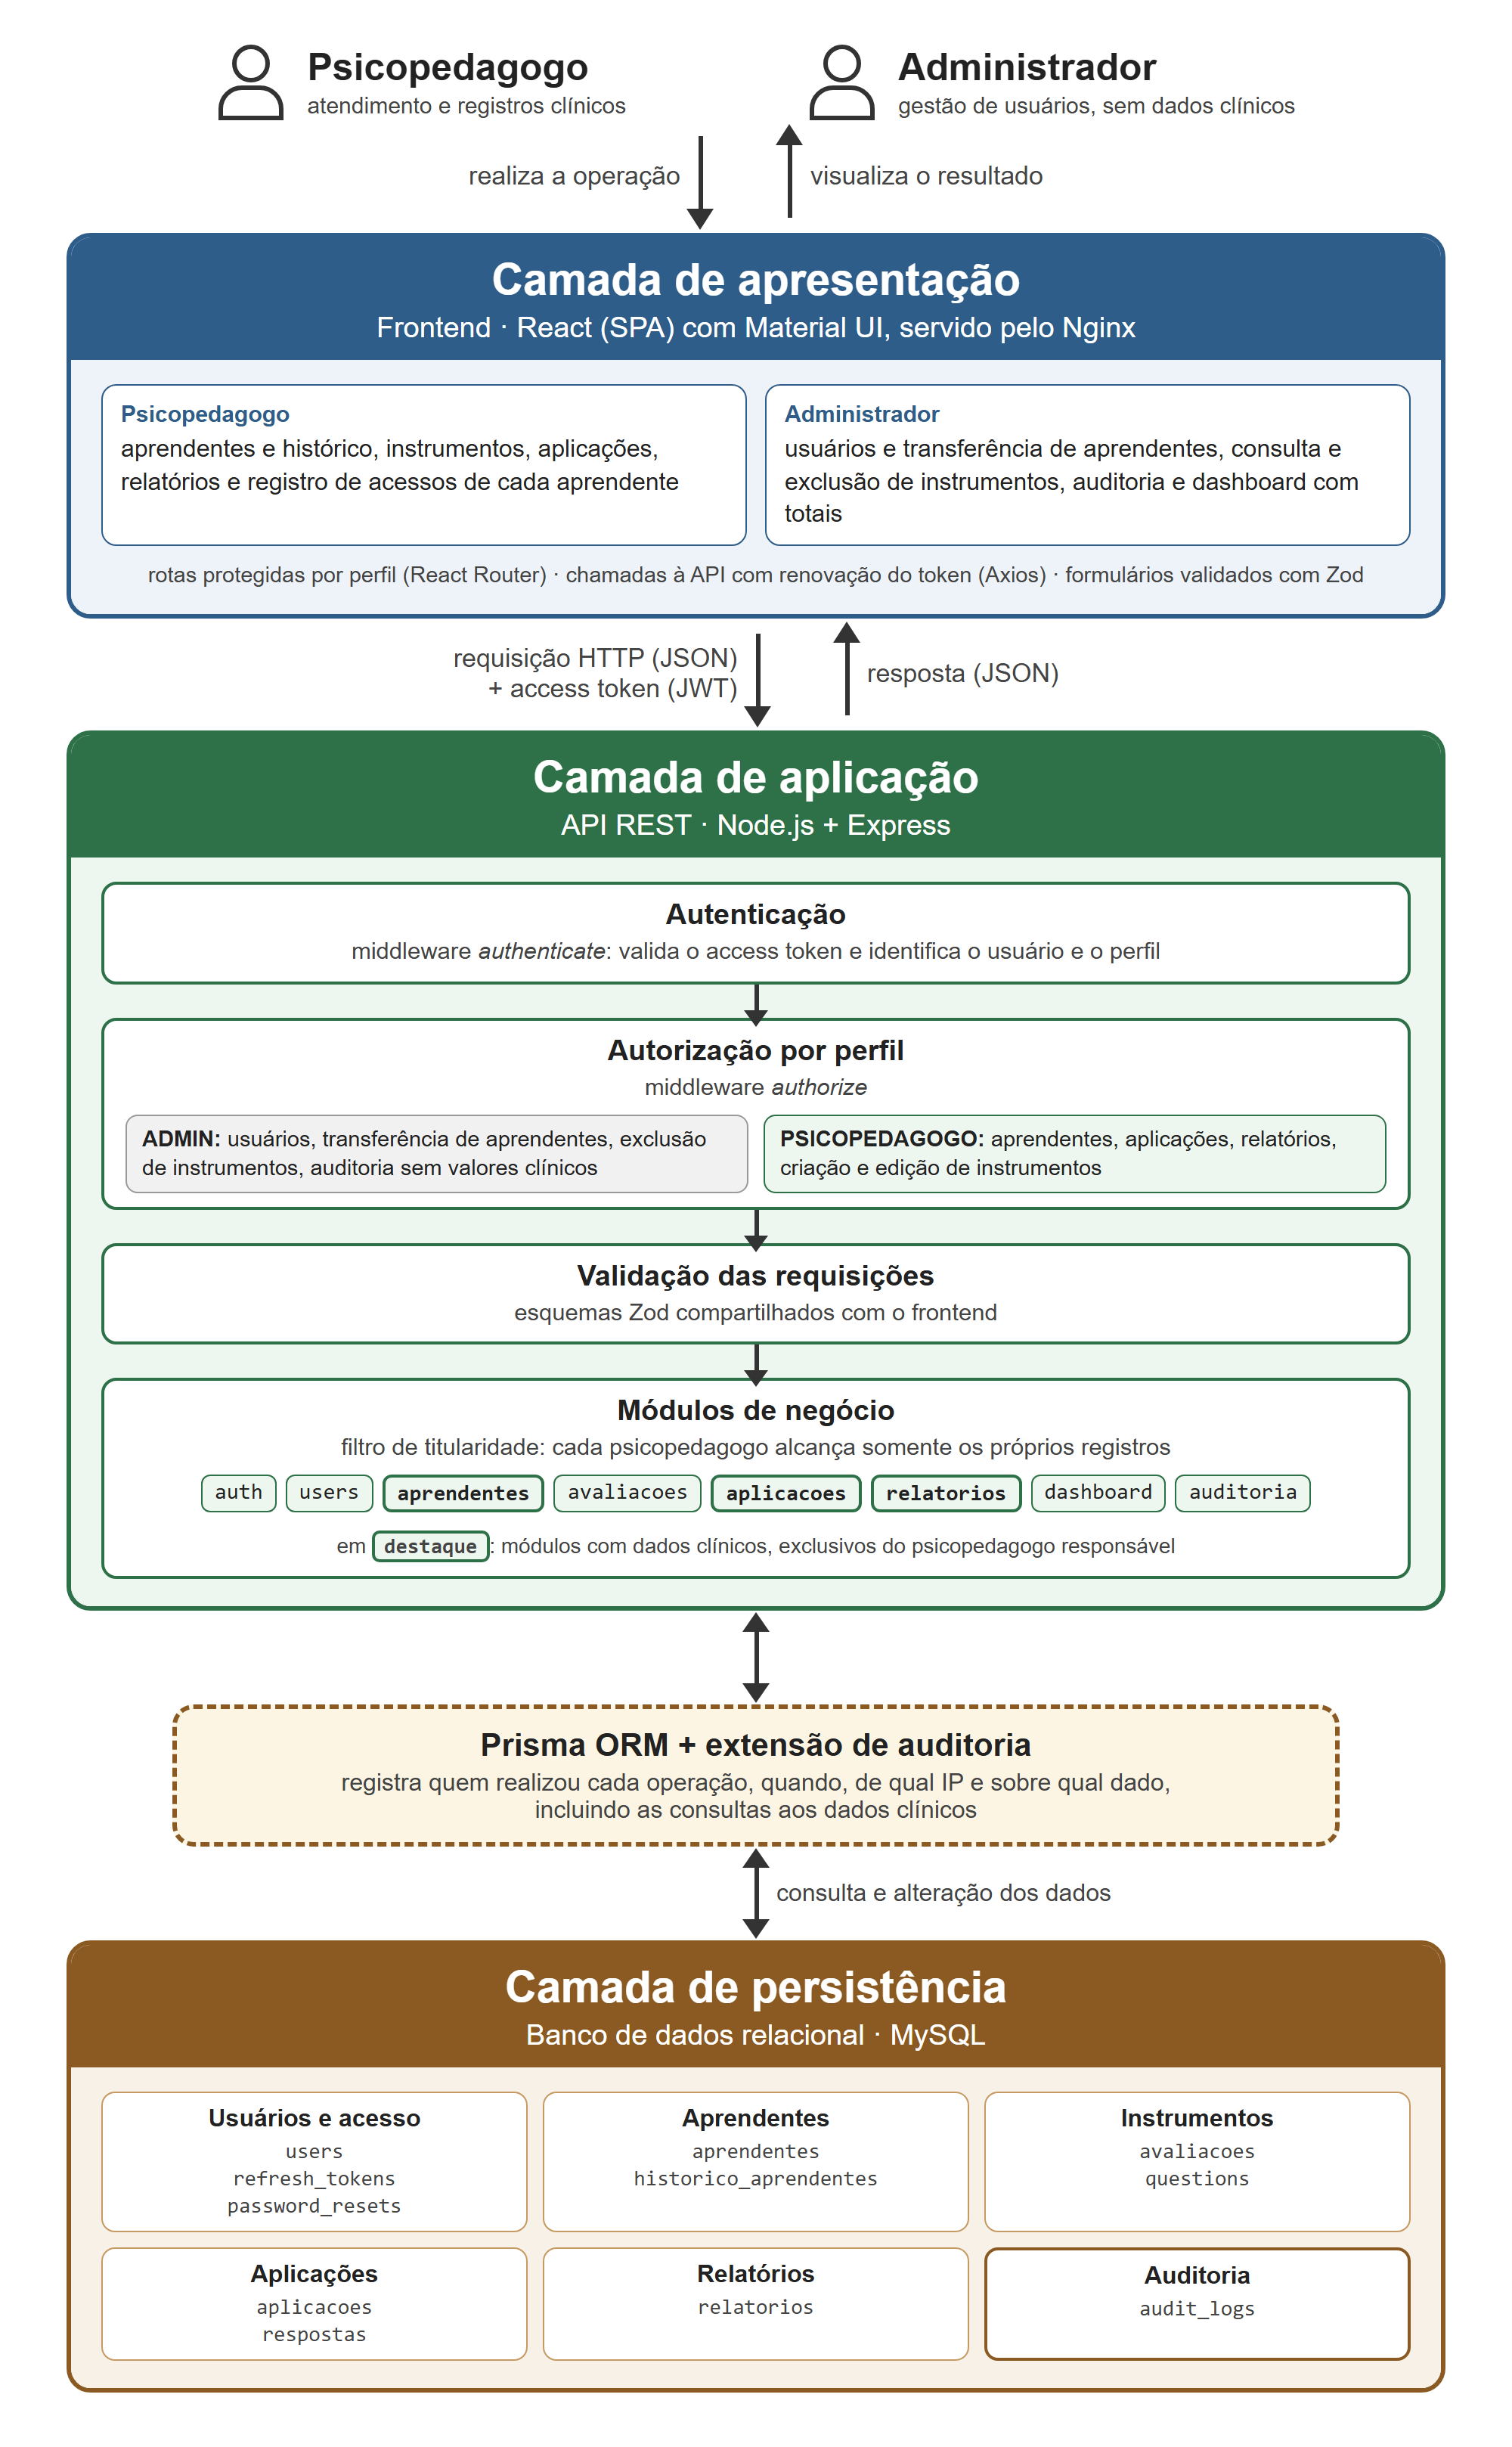
\includegraphics[height=0.78\textheight,keepaspectratio]{figuras/arquitetura_sistema.png}
\end{column}
\begin{column}{0.58\textwidth}
\begin{itemize}
    \small
    \item Três camadas: apresentação, aplicação e persistência.
    \item Requisições passam por autenticação, autorização e validação antes dos módulos.
    \item 8 módulos de negócio independentes.
    \item MySQL com 11 tabelas, acessado pelo Prisma.
    \item Serviços em contêineres Docker; Nginx como \textit{proxy} reverso.
\end{itemize}
\end{column}
\end{columns}
\end{frame}

\begin{frame}{Segurança e Controle de Acesso}
\begin{itemize}
    \small
    \item \textbf{Perfil (RBAC):} \textit{ADMIN} e \textit{PSICOPEDAGOGO}.
    \item \textbf{Titularidade:} cada psicopedagogo vê apenas os próprios aprendentes e instrumentos; aplicações e relatórios herdam a titularidade da criança.
    \item \textbf{Separação entre administração e dados clínicos:} o administrador gerencia contas, mas não acessa avaliações nem relatórios (Código de Ética do Psicopedagogo, art. 7º e 9º).
    \item \textbf{Transferência} de aprendentes entre profissionais para garantir a continuidade.
    \item \textbf{Auditoria} de criações, alterações, exclusões e consultas.
    \item JWT com renovação, senhas com bcrypt e limitação de requisições.
\end{itemize}
\end{frame}

\begin{frame}{Versionamento dos Instrumentos}
\centering
\begin{tikzpicture}[
    inst/.style={draw, rounded corners, minimum width=2.6cm, minimum height=0.9cm, align=center, font=\small},
    apl/.style={draw, fill=gray!15, rounded corners, minimum width=1.6cm, minimum height=0.6cm, font=\footnotesize},
    seta/.style={->, thick}
]
    \node[inst] (v1) at (0,0) {Instrumento v1\\\textit{ARCHIVED}};
    \node[inst, fill=green!15] (v2) at (6,0) {Instrumento v2\\\textit{ACTIVE}};
    \draw[seta] (v1) -- node[above, font=\footnotesize] {edição das questões} node[below, font=\footnotesize] {(já aplicado)} (v2);

    \node[apl] (a1) at (-1,-1.8) {Aplicação 1};
    \node[apl] (a2) at (1,-1.8) {Aplicação 2};
    \node[apl] (a3) at (6,-1.8) {Aplicação 3};
    \draw[seta] (a1) -- (v1);
    \draw[seta] (a2) -- (v1);
    \draw[seta] (a3) -- (v2);
\end{tikzpicture}

\vspace{0.4cm}
\raggedright
\begin{itemize}
    \small
    \item Sem aplicações vinculadas, a edição é salva no próprio registro.
    \item Com aplicações, o sistema arquiva a versão atual e cria uma nova.
    \item Cada aplicação e relatório mantém a versão efetivamente utilizada.
\end{itemize}
\end{frame}

\begin{frame}{Telas do Sistema: Painel e Editor de Instrumentos}
\begin{columns}[c]
\begin{column}{0.5\textwidth}
\centering
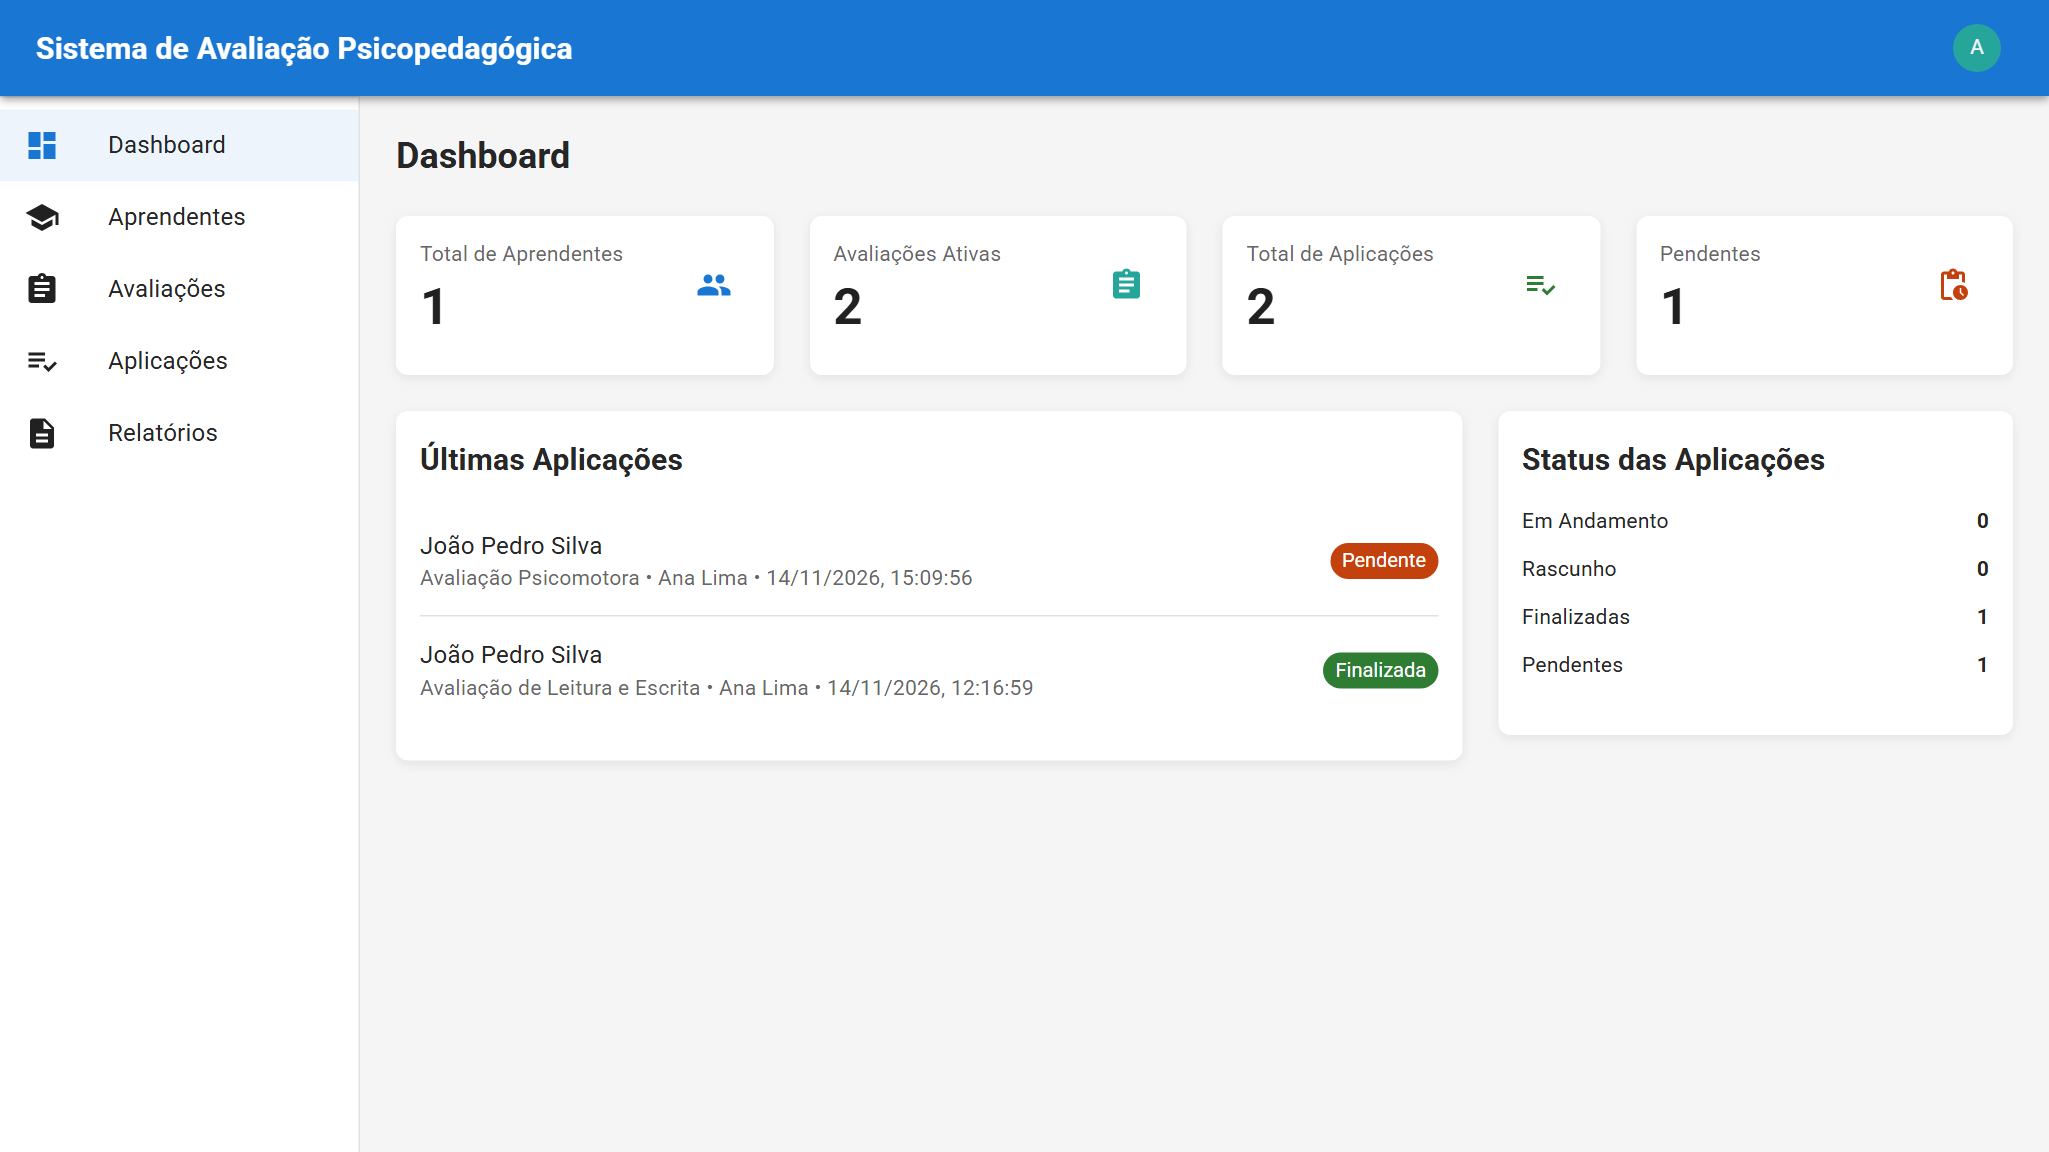
\includegraphics[width=\textwidth]{figuras/tela_dashboard.png}\\
\footnotesize Painel inicial
\end{column}
\begin{column}{0.5\textwidth}
\centering
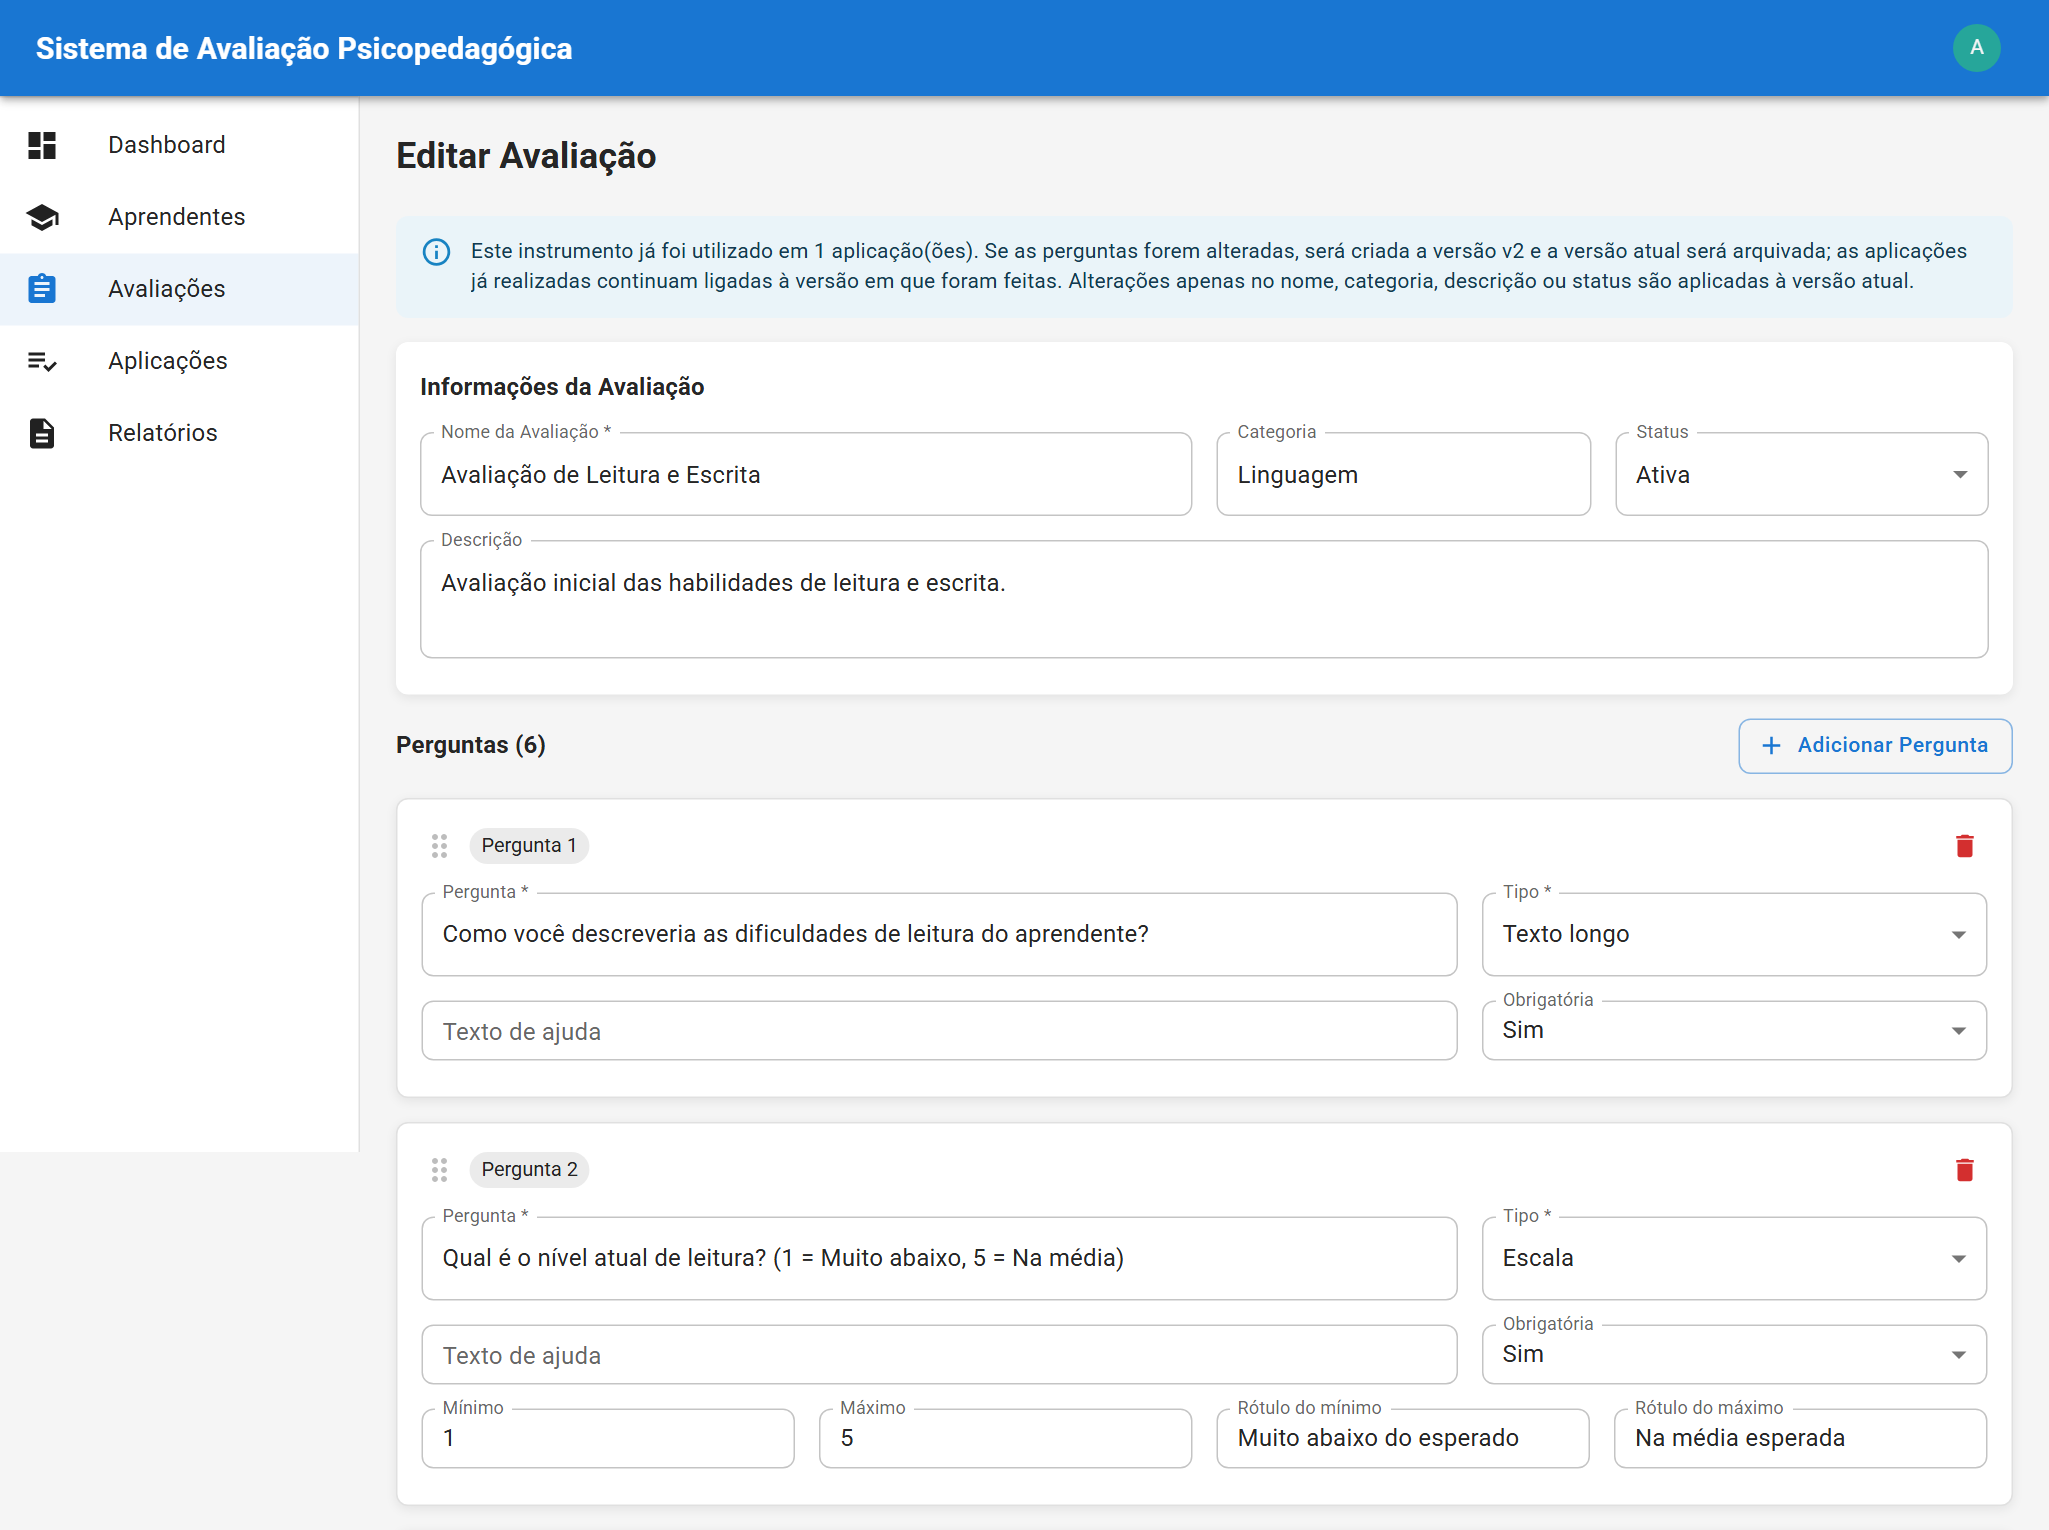
\includegraphics[width=\textwidth]{figuras/tela_instrumento_editor.png}\\
\footnotesize Editor de instrumentos
\end{column}
\end{columns}
\end{frame}

\begin{frame}{Telas do Sistema: Aplicação e Relatório}
\begin{columns}[c]
\begin{column}{0.6\textwidth}
\centering
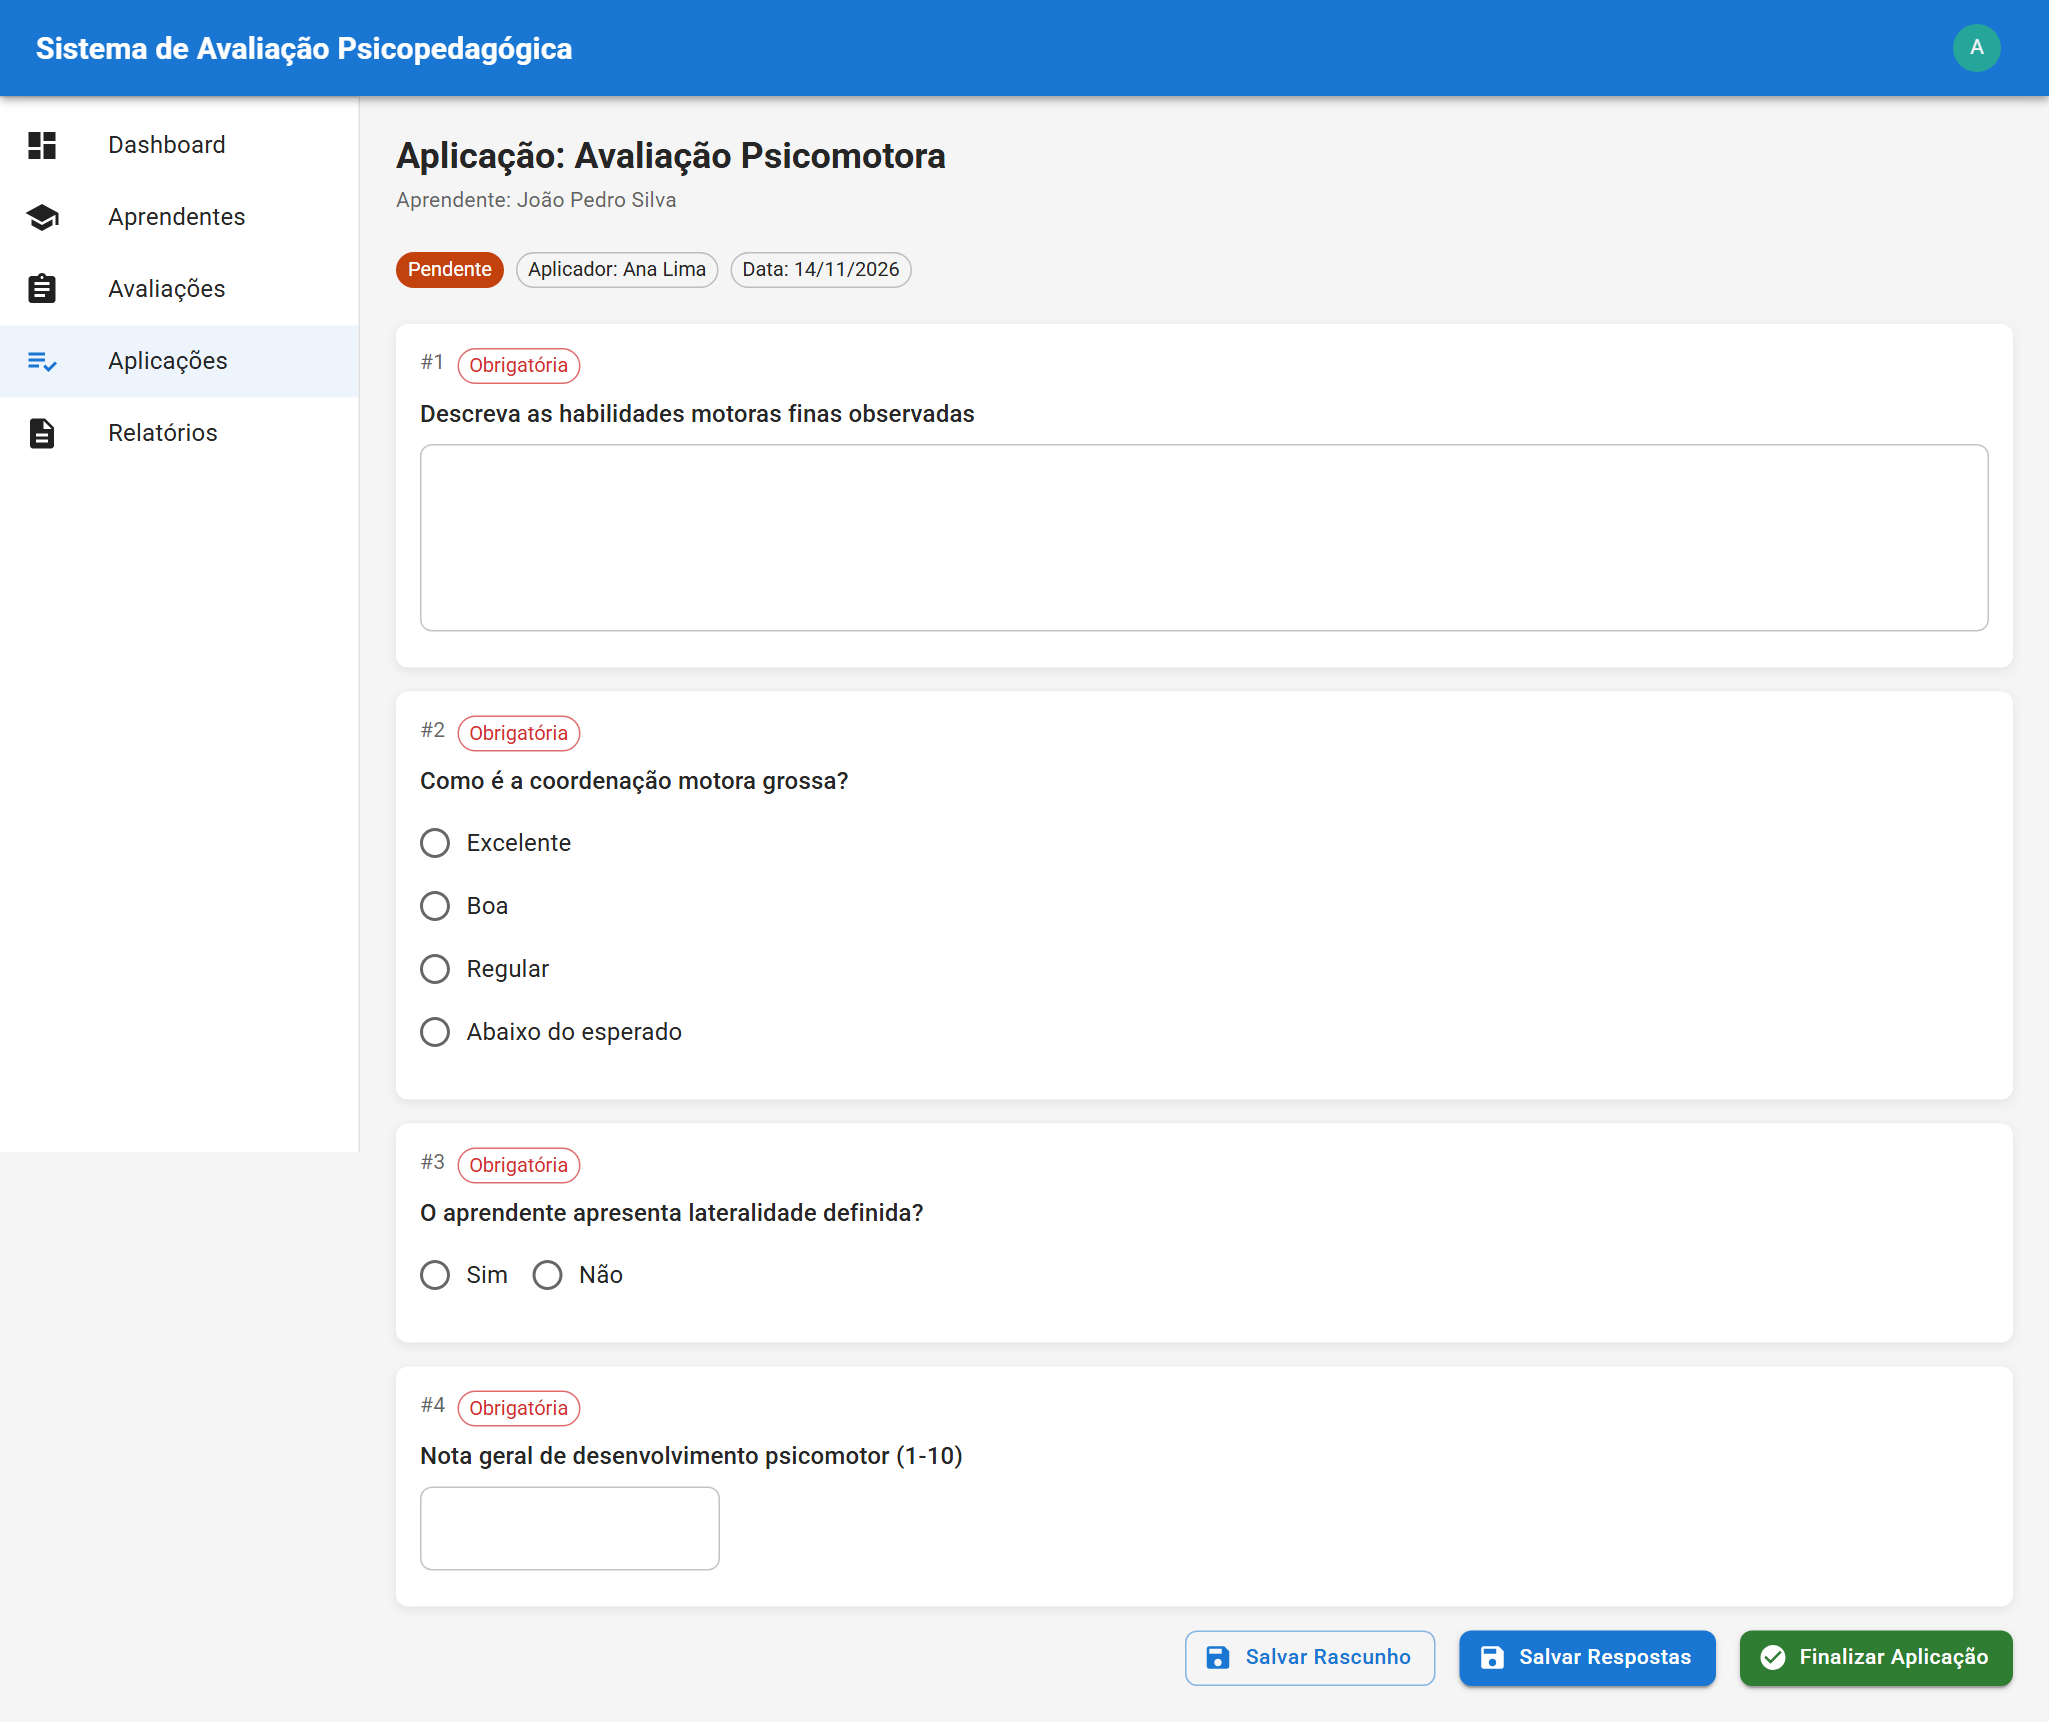
\includegraphics[width=\textwidth]{figuras/tela_aplicacao.png}\\
\footnotesize Preenchimento da aplicação
\end{column}
\begin{column}{0.4\textwidth}
\centering
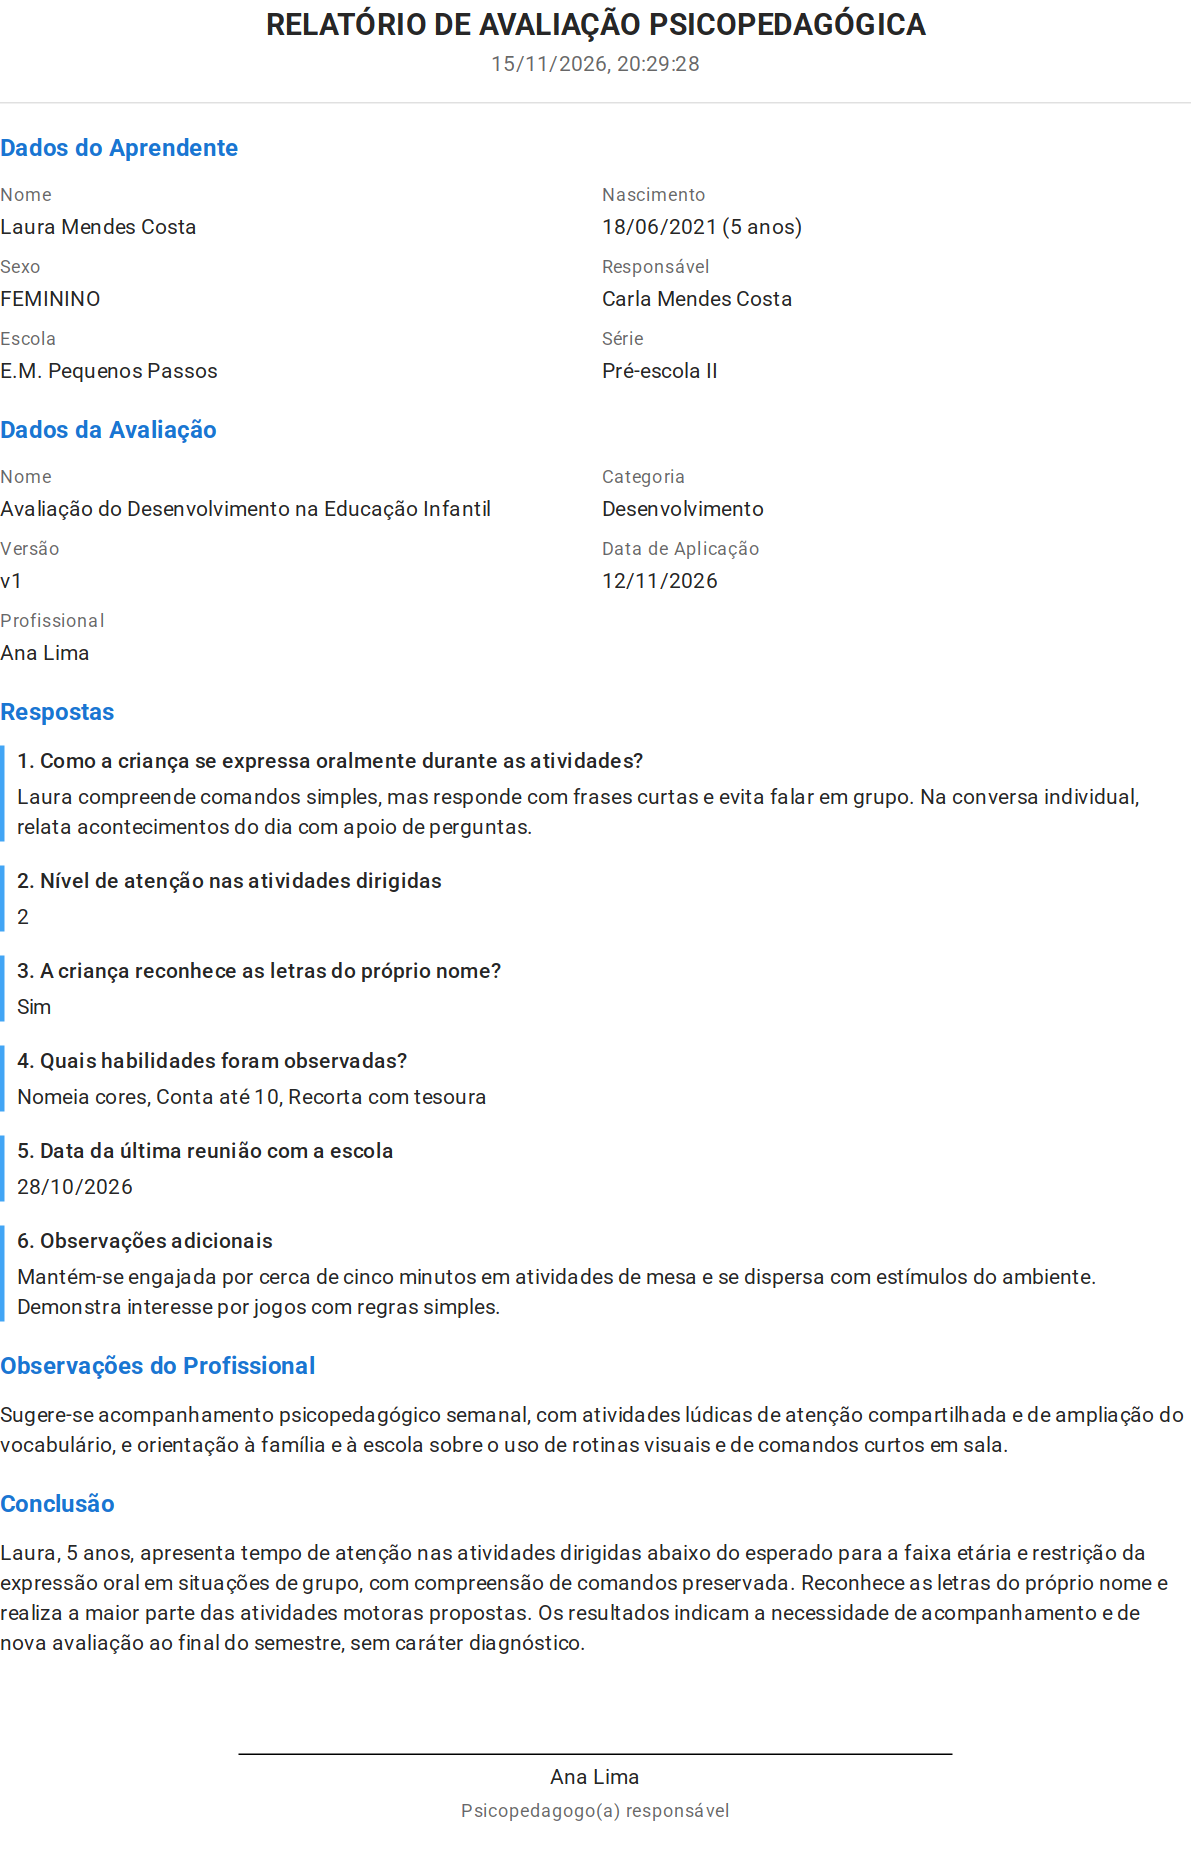
\includegraphics[height=0.68\textheight,keepaspectratio]{figuras/tela_relatorio_impresso.png}\\
\footnotesize Relatório impresso em PDF
\end{column}
\end{columns}
\end{frame}

%%%%%%%%%%%%%%%%%%%%%%%%%%%%%%%%%%%%%%%%%%%%%%%%%%%%%%%%
\section{Resultados e Discussões}
%%%%%%%%%%%%%%%%%%%%%%%%%%%%%%%%%%%%%%%%%%%%%%%%%%%%%%%%

\begin{frame}{Atendimento aos Requisitos}
\begin{itemize}
    \item \textbf{Funcionais:} 13 de 15 atendidos; 2 parcialmente.
    \begin{itemize}
        \small
        \item RF09: adaptações versionadas, mas sem campo de justificativa.
        \item RF12: aplicações e relatórios não integrados à página do aprendente.
    \end{itemize}
    \item \textbf{Não funcionais:} 10 de 11 atendidos; 1 parcialmente.
    \begin{itemize}
        \small
        \item RNF03: sem criptografia em repouso e sem política de retenção.
    \end{itemize}
\end{itemize}
\end{frame}

\begin{frame}{Testes e Acessibilidade}
\begin{columns}[T]
\begin{column}{0.5\textwidth}
\textbf{Testes automatizados}
\begin{itemize}
    \small
    \item 147 testes aprovados (88 \textit{backend}, 59 \textit{frontend}).
    \item Cobertura de linhas: 83,06\% no \textit{backend} (meta: 70\%).
    \item Fluxo completo verificado no ambiente Docker.
\end{itemize}
\end{column}
\begin{column}{0.5\textwidth}
\textbf{Acessibilidade (axe-core)}
\begin{itemize}
    \small
    \item 18 telas, critérios A e AA das WCAG 2.2.
    \item 5 tipos de violação, 2 críticos, todos corrigidos.
    \item Nova execução sem violações.
    \item Verificação apenas automatizada.
\end{itemize}
\end{column}
\end{columns}
\end{frame}

\begin{frame}{Avaliação com Profissionais}
\small
Cinco psicopedagogas, uso livre por cerca de 30 minutos, questionário anônimo (escala de 1 a 5):
\vspace{0.1cm}

\centering
\begin{tikzpicture}
\begin{axis}[
    xbar,
    width=0.8\textwidth,
    height=0.62\textheight,
    xmin=1, xmax=5,
    xtick={1,2,3,4,5},
    symbolic y coords={rel,inst,apl,fac,org,contr,apr},
    ytick=data,
    yticklabels={Relatórios,Instrumentos,Aplicações,Facilidade de uso,Organização,Contribuição geral,Aprendentes},
    yticklabel style={font=\footnotesize},
    xticklabel style={font=\footnotesize},
    nodes near coords,
    nodes near coords style={font=\footnotesize},
    /pgf/number format/use comma,
    bar width=8pt,
    enlarge y limits=0.1,
]
\addplot[fill=gray!50] coordinates {
    (3.8,rel)
    (4.2,inst)
    (4.4,apl)
    (4.6,fac)
    (4.6,org)
    (4.6,contr)
    (4.8,apr)
};
\end{axis}
\end{tikzpicture}

\raggedright
Média geral: \textbf{4,43}; 94,3\% das respostas com notas 4 ou 5.
\end{frame}

\begin{frame}{Discussão}
\begin{itemize}
    \small
    \item A menor média (relatórios) coincide com as sugestões: seções para hipótese diagnóstica e encaminhamentos, anexos e linha do tempo do aprendente.
    \item Interesse das profissionais pelo acompanhamento longitudinal do processo.
    \item Valgas (2021): também DSR e usabilidade positiva, mas com pontuação automática de testes, ausente neste sistema.
    \item TEDI e ASQ-3 oferecem instrumentos validados fixos; este sistema permite cadastrar e adaptar instrumentos com histórico de versões.
    \item Respostas estruturadas e relatórios em texto livre respondem à tensão apontada por Kariotis et al. (2022).
\end{itemize}
\end{frame}

%%%%%%%%%%%%%%%%%%%%%%%%%%%%%%%%%%%%%%%%%%%%%%%%%%%%%%%%
\section{Conclusão}
%%%%%%%%%%%%%%%%%%%%%%%%%%%%%%%%%%%%%%%%%%%%%%%%%%%%%%%%

\begin{frame}{Conclusão}
\begin{itemize}
    \item O objetivo geral foi alcançado: sistema web funcional que cobre o fluxo do cadastro do aprendente ao relatório.
    \item Os seis objetivos específicos foram atendidos, alguns com ressalvas (LGPD e acessibilidade).
    \item \textbf{Contribuição:} o instrumento avaliativo como elemento central, com cadastro pelo profissional e versionamento vinculado às aplicações.
    \item Sistema percebido como adequado à prática profissional, mas ainda em estágio de protótipo.
\end{itemize}
\end{frame}

\begin{frame}{Limitações}
\begin{itemize}
    \small
    \item Sem criptografia em repouso, registro de consentimento, base legal e política de retenção: \textbf{não pode ser usado com dados reais}.
    \item Auditoria fora da transação e sem proteção contra alteração direta no banco.
    \item Sem interoperabilidade (HL7 FHIR, CSV estruturado).
    \item Executado apenas em ambiente Docker local.
    \item Avaliação com cinco participantes e questionário não padronizado; requisitos baseados em uma única entrevista.
\end{itemize}
\end{frame}

\begin{frame}{Trabalhos Futuros}
\begin{itemize}
    \small
    \item Adequação à LGPD: criptografia, HTTPS, consentimento, retenção e descarte.
    \item Linha do tempo na página do aprendente e justificativa das adaptações.
    \item Regras de pontuação automática nos instrumentos.
    \item Relatórios com seções predefinidas e anexos (laudos, pareceres).
    \item Testes manuais de acessibilidade e com pessoas com deficiência.
    \item Nova avaliação com amostra maior, em produção e com a SUS.
\end{itemize}
\end{frame}

\begin{frame}[standout]
  Obrigada!
\end{frame}

\end{document}
